%%%%%%%%%%%%%%%%%%%%%%%%%%%%%%%%%%%%%%%%%%%%%%%%%%%%%%%%%%%%%%%%%%
%%%%%%%% ICML 2014 EXAMPLE LATEX SUBMISSION FILE %%%%%%%%%%%%%%%%%
%%%%%%%%%%%%%%%%%%%%%%%%%%%%%%%%%%%%%%%%%%%%%%%%%%%%%%%%%%%%%%%%%%
\documentclass{article}
\usepackage{times}
\usepackage{graphicx} % more modern
\usepackage{subfigure} 
% For citations
\usepackage{natbib}
% For algorithms
\usepackage{algorithm}
\usepackage{algorithmic}

% Stuff that I added in (Daniel Seita) 
\usepackage{amsmath,amssymb,amsthm,enumitem,verbatim}
\graphicspath{ {Images/} }
\newtheorem{thm}{Theorem}[section]
\newtheorem{conj}[thm]{Conjecture}
\newtheorem{cor}[thm]{Corollary}
\newtheorem{lem}[thm]{Lemma}
\newtheorem{prop}[thm]{Proposition}
\newtheorem{exa}[thm]{Example}
\newtheorem{defi}[thm]{Definition}
\newtheorem{exe}[thm]{Exercise}
\newtheorem{rek}[thm]{Remark}
\newtheorem{que}[thm]{Question}
\newtheorem{prob}[thm]{Problem}
\newtheorem{cla}[thm]{Claim}
% End of stuff I added in

% As of 2011, we use the hyperref package to produce hyperlinks in the resulting PDF.  If this breaks your system, please commend out the following
% usepackage line and replace \usepackage{icml2014} with \usepackage[nohyperref]{icml2014} above.
\usepackage{hyperref}

% Packages hyperref and algorithmic misbehave sometimes.  We can fix this with the following command.
\newcommand{\theHalgorithm}{\arabic{algorithm}}

% Employ the following version of the ``usepackage'' statement for submitting the draft version of the paper for review.  This will set the note in
% the first column to ``Under review.  Do not distribute.''
%\usepackage{icml2014} 
% Employ this version of the ``usepackage'' statement after the paper has been accepted, when creating the final version.  This will set the note in
% the first column to ``Proceedings of the...''
\usepackage[accepted]{icml2014}

% The \icmltitle you define below is probably too long as a header.  Therefore, a short form for the running title is supplied here:
\icmltitlerunning{The Distributed Retired Traveling Salesman Problem}

\begin{document} 

\twocolumn[
\icmltitle{The Distributed Retired Traveling Salesman Problem}

% It is OKAY to include author information, even for blind submissions: the style file will automatically remove it for you unless you've provided the
% [accepted] option to the icml2014 package.
\icmlauthor{Daniel Seita}{dts1@williams.edu}
\icmlauthor{Ziang Zhang}{zz2@williams.edu}
\icmladdress{Department of Computer Science, Williams College, Williamstown, MA 01267 USA}

% You may provide any keywords that you find helpful for describing your paper; these are used to populate the "keywords" metadata in the PDF but will
% not be shown in the document
\icmlkeywords{distributed systems}

\vskip 0.3in
]

\begin{abstract} 
The use of major online travel agencies has made scheduling long-term travel much easier by allowing users to easily identify a set of flights in just
a few clicks. Current travel agencies allow users to plan out long-term trips involving flights to more than two cities, but they require specific
arrival and departure dates for each city and a city ordering. We present a system that does not burden the user with these decisions. Specifically,
our code takes in two required inputs: a list of cities the user wishes to travel to, and a date range over which they are willing to travel, and
outputs the cheapest set of flights within that range that form a valid route. It essentially solves a harder version of the Traveling Salesman
Problem since costs are not constant between two cities. Under several weak assumptions, and assuming that the number of cities and days is
sufficiently limited, then our algorithm should successfully find the cheapest cost flight in a reasonable amount of time. We present the theoretical
and systematic components of the project and discuss empirical results.
\end{abstract} 

\section{Introduction and Motivation}\label{sec:intro}

The use of major online travel agencies, such as Travelocity\footnote{\url{www.travelocity.com}} and Kayak\footnote{\url{www.kayak.com}}, has made
scheduling long-term travel much easier by allowing users to easily select a set of flights to purchase tickets from. People use a combination of
factors to help them make their decision, such as the total price of the flights and the days they wish to land and depart from a city. Current travel
agencies allow users to plan out trips involving airlines to multiple destinations (see Figure~\ref{fig:travelocity} for an example using
Travelocity), but they require (1) specific dates for each city and (2) an ordering.

This limitation can make searching for flight routes time-consuming for users who are not restricted to arriving at cities on particular dates. For
instance, suppose one resides in New York City (NYC) and wants to schedule a summer trip to Paris, London, and Tokyo from June 1 to June 20, and it
does not matter to him how long he stays in a city. Suppose that it also does not matter the ordering that he arrives at the cities. Thus (for now) we
will only care about the following factors\footnote{For brevity, we list a high-level overview of the problem without getting into too many technical
details; Section~\ref{sec:limitations} describes some of our assumptions and limitations.}:

\begin{itemize}[noitemsep]
    \item The full flight route occurs within the date range (in this case, between June 1 and June 20).
    \item The flight route must arrive and leave at least once for NYC, Paris, London, and Tokyo.
    \item The flight route is valid and logically consistent. For instance, if the first flight takes him from NYC to Tokyo, the second flight in the
    route should not depart from a place other than Tokyo.
\end{itemize}

There are a vast pool of valid flight routes. We might assume that out of all these, one would want the \emph{cheapest} route. Of course, this glosses
over how the user may want to spend some number of days at each city, but this is the most general case.

Unfortunately, finding the cheapest route possible is challenging using current agencies, because they require knowing the arrival and departure dates
for each city. The reason for this is simple: the problem of finding this flight route is a hard problem to solve. In fact, this problem is very
similar to the well-known Traveling Salesman Problem~\cite{Applegate:2007:TSP:1374811}, which asks if there exists a cycle in a graph that touches
each node exactly once (i.e., a Hamiltonian cycle). Each edge has a cost associated with it, and the decision version of the problem, which asks if
there exists a valid Hamiltonian cycle with cost bounded by $B$, is NP-complete~\cite{Kar72}. In our case, we do not force the user to visit each
city exactly once because the cheapest flight through a sequence of cities \emph{may require} visiting a city more than once.

What makes our problem (likely) much harder than the Traveling Salesman Problem is that the cost of an edge between two nodes in our graph (i.e., two
cities) is not constant, because flight prices frequently change. We coin our problem the ``Distributed Retired Traveling Salesman Problem.'' The
``Retired'' portion comes from how we assume that whoever is planning this trip is retired, because otherwise, how would he or she have the time and
money? The ``Distributed'' part is because we incorporate concepts from the design and practice of distributed systems to build software that can
tackle this problem. We discuss the mathematical and systems portions of our solution in Sections~\ref{sec:math} and~\ref{sec:systems}, respectively.

\begin{figure}[t]
\vskip 0.2in
\begin{center}
\centerline{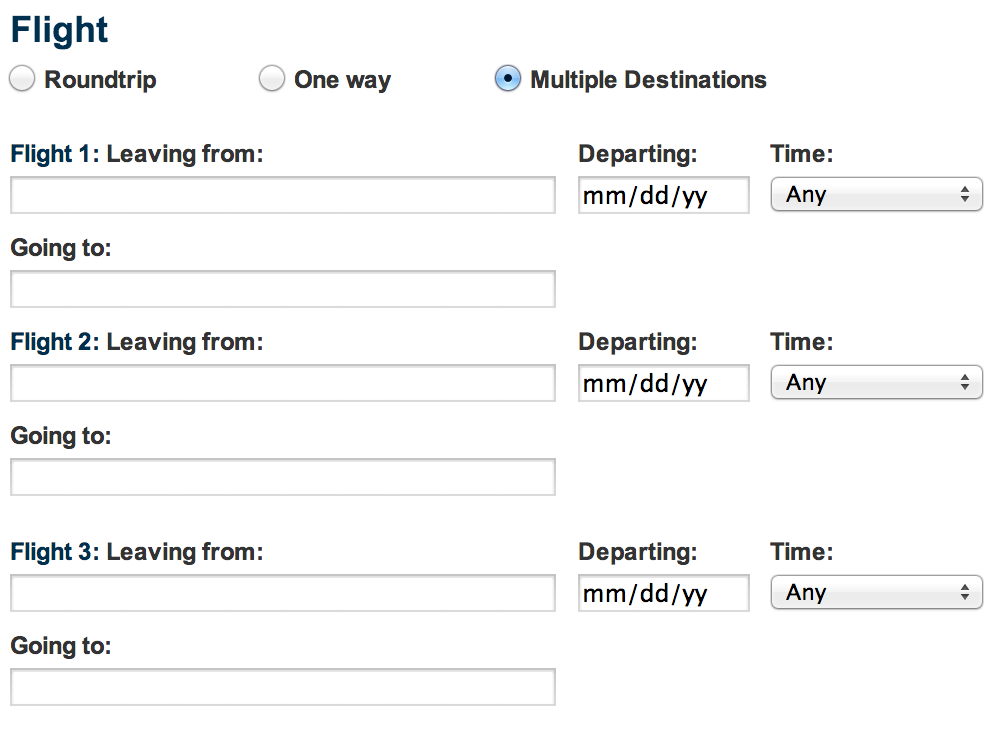
\includegraphics[width=\columnwidth]{travelocity}}
\caption{Travelocity lets users select multiple destinations.}
\label{fig:travelocity}
\end{center}
\vskip -0.2in
\end{figure}

\section{Related Work}\label{sec:related_work}

The Traveling Salesman Problem (TSP) is one of the oldest and most well-known problems in combinatorial optimization. While no exact, polynomial time
solution for the decision problem is known, there is a $3/2$-approximation algorithm due to Christofides~\cite{Chr76}. That algorithm was long the
standard approximation algorithm until a stunning recent result in~\cite{conf/focs/GharanSS11}, which has thus spurred a cascade of additional
research relating to the TSP (e.g.,~\cite{Moemke:2011:AGT:2082752.2082898}).

In contrast to the attention devoted to TSP, there appears to be very little research focusing on the special case of our problem, which introduces
additional challenges. These can be mathematically-oriented, such as how to manage the variable costs, or systems-oriented, such as how to even obtain
the actual flight costs. We have found nothing in the literature that particularly fits our problem.

\section{Mathematical Component}\label{sec:math}

The mathematical portion of our work uses a technique known as \emph{binary integer linear programming}, which falls under the broader category of
optimization techniques. The goal in optimization is straightforward: given a set of variables and a set of constraints, the goal is to find the best,
feasible solution according to some criteria, such as cost (in which case, ``best'' means ``minimal'').

\subsection{Linear and Integer Programming}\label{sec:lin_int_programming}

One of the most commonly-used optimization techniques is linear programming, introduced by Dantzig in~\cite{GVK180926950}.

\begin{defi}\label{defi:linear_programming}
A \emph{linear programming problem} consists of three components: 
\begin{enumerate}[noitemsep]
    \item a finite collection of linear inequalities or equations in a finite number of unknowns, $x_1, \ldots, x_n$;
    \item sign constraints $x_i \ge 0$ on some (possibly empty) subset of the unknowns;
    \item a linear function to be minimized or maximized.
\end{enumerate}
An assignment to the variables $x_1, \ldots, x_n$ satisfying the first two conditions is a \emph{feasible} solution. If it also satisfies the third,
then it is an \emph{optimal} solution~\cite{opac-b1105716}.
\end{defi}

Linear programming has tremendous applications, and a full list of them would be impossible to create. Some problems well-suited to linear programming
include investment management, scheduling problems, and the diet problem. (The last problem concerns the rather interesting question of what is the
minimum cost of a nutritionally adequate diet.) The reason for linear programming's great versatility is the ease at which constraints can be added to
a model.

More specific cases of linear programming are integer and binary linear programming. (Sometimes we drop the ``linear'' part for brevity.)

\begin{defi}\label{defi:integer_programming}
An \emph{integer programming problem} is a linear programming problem with the added restriction that all variables (i.e., unknowns) $x_1, \ldots,
x_n$ are integers.
\end{defi}

\begin{defi}\label{defi:binary_programming}
A \emph{binary integer programming problem} is an integer programming problem with the added restriction that all variables $x_1, \ldots,
x_n$ are such that $x_i \in \{0,1\}$.
\end{defi}

We see that our problem is particularly suited to binary integer programming, because all the possible flights we could take can be viewed as a set of
binary random variables, each of which has value 1 if we decide to take that flight, and 0 otherwise. We now formulate this problem in more detail.

\subsection{An Integer Programming Formulation}\label{sec:int_prog_form}

To start formulating the problem, we make it concrete what we mean by cities, days, and costs.

\begin{itemize}[noitemsep]
    \item We have $n$ cities to reach; we index cities by $i$ or $j$, where $i, j \in \{1, 2, \ldots, n\}$.
    \item We have $t$ consecutive days when we can travel: $t \in \{1, 2, \ldots, m\}$.
    \item The minimum cost for traveling from city $i$ to $j$ on day $t$ is $c_{ijt}$.
\end{itemize}

Using the above lets us define the following variables:

\[
x_{ijt} = \begin{cases}
1 &\mbox{if we go from cities } i \mbox{ to } j \mbox{ on day } t, \\ 
0 & \mbox{otherwise}.
\end{cases}
\]

Thus, a solution to our problem will be the full assignment to each of the above variables. The set of the binary variables that equal one will
(assuming the set has cardinality $k$) correspond to $k$ flights $f_1, \ldots, f_k$ ordered by date.

For now, we make several simplifying assumptions, and defer a more detailed discussion about the realism of this project in
Section~\ref{sec:limitations}. Perhaps the most important one is that we assume each flight is assigned to exactly one day. We will also force a valid
solution to have flights all on different days. This means, at the moment, we do not consider issues related to (1) overnight flights (we will pretend
they do not exist), (2) multiple-stop flights on the same day, and (3) possible logistic impossibilities such as flight $f_i$ arriving at 11:59 PM and
then the next flight $f_{i+1}$ departing from the same airport two minutes later (but on the next day).

The goal is to solve this minimization problem:

\begin{equation}
\mbox{Minimize } \sum_{t=1}^{m} \sum_{i=1}^{n} \sum_{j=1}^{n} c_{ijt}x_{ijt},
\end{equation}

\emph{subject to} the following constraints:
\begin{align}
\sum_{i=1}^{n} \sum_{j=1}^{n} x_{ijt} &\le 1 \mbox{ for all } t \in \{1, 2, \ldots, m\}, \\ 
\sum_{t=1}^{m} \sum_{i=1}^{n} x_{ijt} &\ge 1 \mbox{ for all } j \in \{1, 2, \ldots, n\}, \\
\sum_{t=1}^{m} \sum_{j=1}^{n} x_{ijt} &\ge 1 \mbox{ for all } i \in \{1, 2, \ldots, n\}.
\end{align}

The first constraint ensures that we have at most one flight per day, which is generally too restrictive for real-life, but will suffice for now. The
second constraint ensures we enter each city at least once. The third constraint ensures we leave each city at least once. These last two reinforce
the notion that going through the cheapest route may mean visiting several cities more than once.

Sadly, these previous constraints are \emph{not} enough to solve our problem. There are two glaring issues with the current constraints that, if we
were to use them to solve this flight scheduling problem, could result in a logically inconsistent flight route.

\subsubsection{Disjoint Cycles}\label{sec:disjoint_cycles}

The first problem is that the constraints do not prevent disjoint cycles. Figure~\ref{fig:bad_solution} shows a graph with six nodes, which may
represent six cities, and a possible edge assignment that is indicative of the route we take to visit all cities. Assuming the flights are all on
different days, the route satisfies our constraints, because we enter and exit each city at least once, but this is not a Hamiltonian cycle.

\begin{figure}[t]
\vskip 0.2in
\begin{center}
\centerline{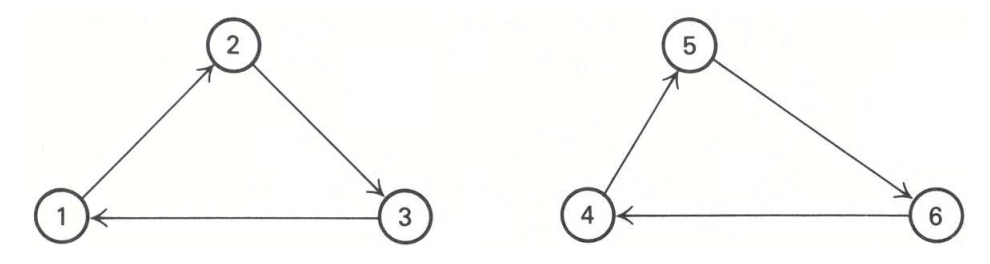
\includegraphics[width=\columnwidth]{bad_solution}}
\caption{This represents two sets of disjoint cycles.}
\label{fig:bad_solution}
\end{center}
\vskip -0.2in
\end{figure}

To prevent disjoint cycles, we need to add additional constraints that correspond to all the ways we can subdivide the cities into two groups so that
both of them contain at least two cities. (A subdivision where one group only has one city is already covered by our earlier constraints since we
would have to leave and enter that city at least once, which requires connecting with the other group.) For instance, with the six-variable situation
in Figure~\ref{fig:bad_solution}, one constraint would be
\begin{align}
\sum_{t=1}^{m} (&x_{14t} + x_{15t} + x_{16t} + x_{24t} + x_{25t} + \\
& x_{26t} + x_{34t} + x_{35t} + x_{36t}) \ge 1, \nonumber
\end{align}

which ensures that at least one leg of the tour connects cities 1, 2, and 3 with cities 4, 5, and 6, so this corresponds to the subdivision of
$\{[1,2,3],[4,5,6]\}$. We can characterize the number of constraints we need to add to prevent disjoint cycles.

\begin{lem}\label{lem:cycle_constraints}
In a problem that has $n \ge 4$ constraints, the number of ways to subdivide the cities so that each has two groups is ${n \choose 2} + {n \choose 3}
+ \cdots + {n \choose n-2}$.
\end{lem}

The reasoning is straightforward: we have two groups, and we want to pick the number of elements for one group. We can pick some number out of $n$
elements to be in one group, and assign all the rest to the others.

One technical note is that the number of constraints from Lemma~\ref{lem:cycle_constraints} can be halved by symmetry. Still, the number of equations
needed grows rapidly with respect to $n$, and the need to implement these various restrictions is why integer programming is a hard task. Integer
programming is, in fact, an NP-hard problem, and the binary case is NP-complete~\cite{Kar72}. In contrast, faster algorithms such as the Simplex
method\footnote{The Simplex Method performs well in practice but its runtime has historically been difficult to evaluate, as in the worst case it
\emph{can} run in exponential time~\cite{Klee1972}. The simplex algorithm has \emph{smoothed complexity} polynomial in the input size; for details
about this, see~\cite{Spielman:2004:SAA:990308.990310}.} are used to solve linear programming problems. Note that simply taking a solution to the
linear programming problem and then rounding it to form a ``solution'' to the integer problem will not work, as we show in Appendix~\ref{app:lin_vs_int}.

\subsubsection{Consecutive Flights in Different Cities}

The second problem with the constraints posed earlier in Section~\ref{sec:int_prog_form}, which the constraints in~\ref{sec:disjoint_cycles} do
\emph{not} resolve, is that we can get flight orderings that are logically inconsistent in the sense that consecutive flights may not agree in their
choice of cities. It makes no sense, for instance, to have flights $f_i$ and $f_{i+1}$ where $f_i$ takes the participant from NYC to Tokyo, and
$f_{i+1}$ takes him or her from Paris to London.

Unfortunately, fixing the flight ordering by adding in constraints is challenging and requires a large number of equations. Our implementation only
adds in one layer of constraints for here, and defers a complete flight logic check to the code that actually generates the tree. Specifically, for
all pairs of days $t$ and cities $c$ such that $t \in \{1,2,\ldots, m-1\}$ and $c \in \{1,2,\ldots,n\}$ we add in the following constraints:
\begin{align}
\underbrace{\left(\sum_{i\ne c} x_{ict} \right)}_{\text{Term 1}} + \underbrace{\left( \sum_{j\ne c}\sum_{k\ne j} x_{jkt^+}\right)}_{\text{Term 2}} \le 1,
\end{align}
% TODO I think it still works for n+1 days but let me think about it and put stuff in the appendix.

where $t^+$ is shorthand for $t+1$ (which explains why we don't set $t$ to be $m$). Term 1 represents entering city $c$, and Term 2 represents leaving
any city other than $c$. Notice that by our previous constraints, both Term 1 and Term 2 are already bounded by one, so if both are one, then this
indicates that two flights on back-to-back days are not logically consistent. We therefore have the following lemma.

\begin{lem}\label{lem:correctness}
Assuming that we have $n$ cities and $n$ days as input, solving the binary integer programming problem using the previous constraints will return a
valid, logically consistent solution.
\end{lem}

Of course, this doesn't prevent the problem of having more days than flights. We resolve that issue by not using constraints at all. We just run the
problem and, each time a candidate solution is proposed, check its complete vector for logical consistency. Appendix~\ref{app:flight_logic} describes
our handling of flight logic in more detail.

\subsection{Using Balas' Additive Algorithm}\label{sec:balas}

To actually solve the binary integer programming problem, we use Balas' Additive Algorithm~\cite{doi:10.1287/opre.13.4.517}. This is a special case of
the larger class of branch-and-bound algorithms, which are used to solve integer programming problems. Branch-and-bound algorithms consist of a
systematic enumeration of all candidate solutions, where large subsets of fruitless candidates are discarded by using upper and lower estimated bounds
of the quantity being optimized~\cite{Clausen1997}.

Balas' algorithm makes use of the special properties of binary integer programming problems. Assuming that the costs are all non-negative, and that
variables are indexed according to cost, we want to (1) set all variables to zero in order to minimize total cost, and (2) if we cannot set all
variables to zero due to constraints, then we wish to set the variable with smallest index to one. What results is a rooted tree where each path of
$n$ nodes from the root indicates an assignment to the first $n$ variables. One can use a standard depth-first search to implement the algorithm.  For
brevity we elide additional technical details of the algorithm and refer the reader to Appendix~\ref{app:balas}.



\section{Systems Component}\label{sec:systems}

We now switch topics and discuss the implementation side. Our code that solves the Distributed Retired Traveling Salesman Problem is made up of
several components that form a multi-tiered client-server model (for an introduction to the client-server model,
see~\cite{Tanenbaum:2006:DSP:1202502}).  We have a front-end server, a master server, and a group of slave servers in the system, as shown in
Figure~\ref{fig:machines}. The slave servers come from machines that we use. Originally, we wanted to use PlanetLab~\cite{conf/osdi/PetersonBFM06},
which is a global platform for deploying and evaluating network services and allows people to use portions of other PlanetLab computers. This was too
complicated to work with, so we stuck with the Williams lab computers.

{\bf TODO We need to fix this up ... and once I get what we're doing here, we can change the slave sever section.}

\begin{figure}[t]
\vskip 0.2in
\begin{center}
\centerline{
\includegraphics[width=\columnwidth]{servers}}
\caption{{\bf TODO. We need to change this.}}
\label{fig:machines}
\end{center}
\vskip -0.2in
\end{figure}

\subsection{Front-end Server}\label{sec:front_end_server}

The front-end server acts as a point of communication between the client\footnote{Somewhat impolitely, we can refer to the set of clients, minus us,
as the ``ignorant masses.''} and our master server. It is a Python script that starts on the command line and outputs introductory messages to the
client so that he or she knows how to use our system. The front-end serve receives user input, forwards the request to the master server (step
\texttt{1} in Figure~\ref{fig:machines}), listens to the master for the result (step \texttt{6}), and displays the result when it is ready. The result
that we print back to the user is currently the single best list of the flights ordered by departure date. If there is more than one optimal solution,
it only returns one of them.

\begin{figure}[t]
\vskip 0.2in
\begin{center}
\centerline{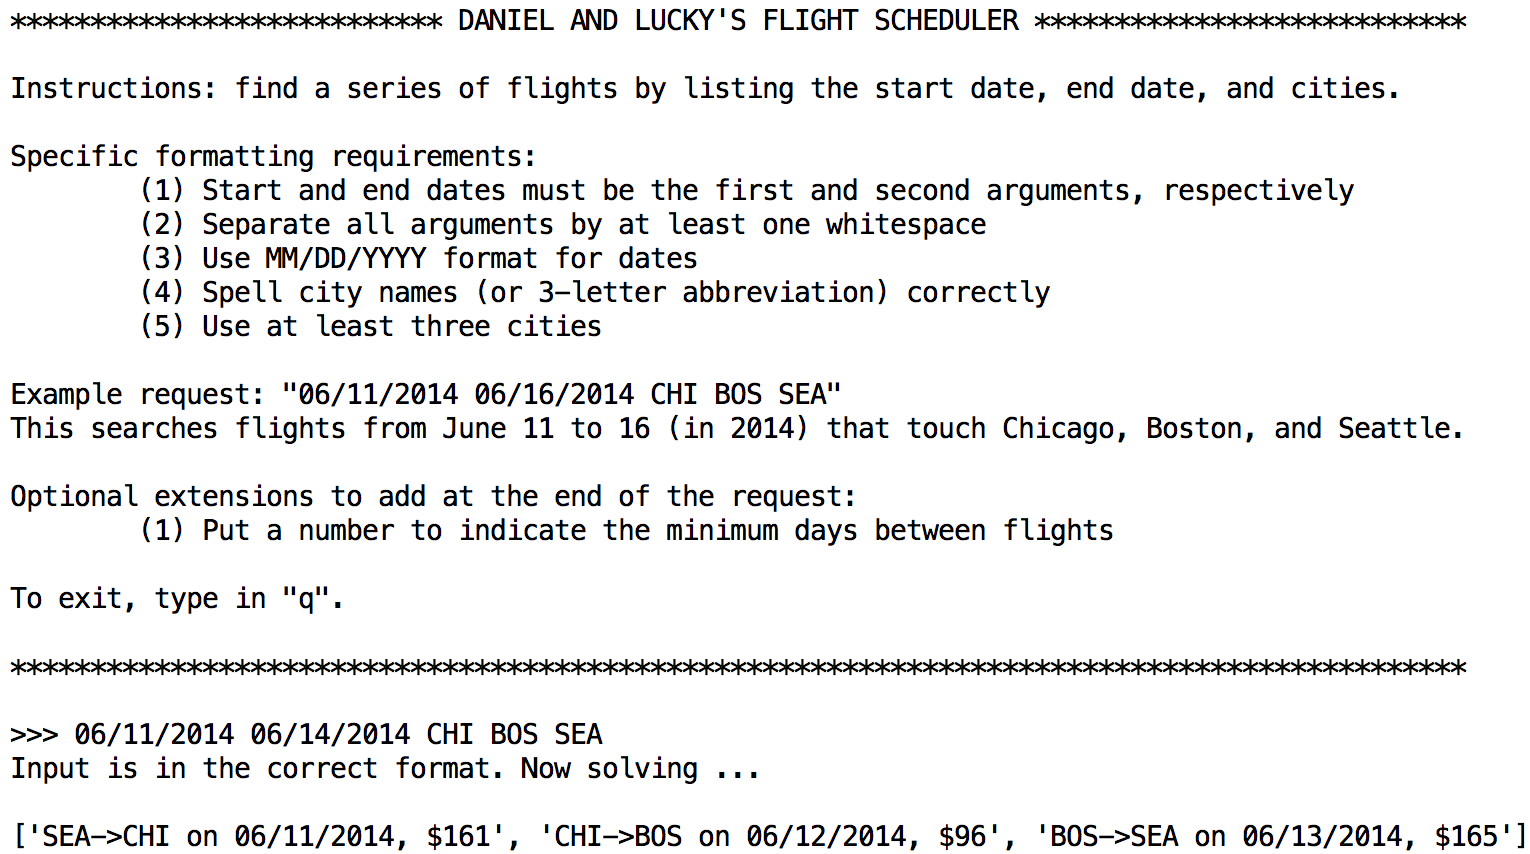
\includegraphics[width=\columnwidth]{front_end_server2}}
\caption{This shows our front-end server.}
\label{fig:front_end_server}
\end{center}
\vskip -0.2in
\end{figure}

Figure~\ref{fig:front_end_server} shows a version of our front-end server (we frequently change its design). Here, the hypothetical user made a
request to find the cheapest flight route that touches Chicago, Boston, and Seattle in the four day period of June 11, 2014 to June 14, 2014.
Our code ran and the master server returned the (valid) flight ordering of Seattle to Chicago, Chicago to Boston, then Boston to Seattle.

Notice that the front-end server has an optional argument where a user can insert a number at the end of their request to indicate the minimum number
of days between any two flights. (The example from Figure~\ref{fig:front_end_server} just happened not to use it.) It is straightforward to add
more of these optional arguments. If time permits, we also plan to transform the command-line interface to a website, which will expand our audience
of potential clients. The front-end server does only minimal checks of the input and defers the parsing to the master server (see
Section~\ref{sec:master_server}).


\subsection{Master Server}\label{sec:master_server}

The master server is the workhorse of our system. It takes in the user request sent in from the front-end server from
Section~\ref{sec:front_end_server}. When a request comes in, the master sever runs a variety of checks and parses the input to make sure that the
request is sound. For instance, given the optional argument where the user can specify the minimum number of days between flights, the server checks
that the full date range is large enough to allow that case to happen. For the full list of checks we implement, see Appendix~\ref{app:input_check}. We
do not catch all possible cases of possible pathological inputs, in part because it is challenging to do so in a command line argument, and also
because we trust our users not to wreck the system. (There has been substantial research in the literature about trust management in systems, such
as~\cite{Blaze:2001:RTM:380171.380186}; for now we eschew these details.)

After parsing the input, the master sever has two important tasks. The first is that it needs to obtain the cheapest flight that goes from cities $i$
to $j$ on day $t$ for all possible combinations of $i, j,$ and $t$ as specified by the user. It accomplishes this by calling the crawler server, also
known as the ``slave server,'' which we discuss in Section~\ref{sec:slave_server}. Once it has all the flights, it proceeds to its next major task,
which is to transform the flight information and user request into inputs suitable for binary integer programming. Computing the cost vector is easy;
the challenging part is making sure that the constraints are well-defined. Once the master sever has computed the necessary constraint matrix, it will
call the binary integer programming solver.  As discussed in Section~\ref{sec:balas}, this runs Balas' Additive Algorithm to create the final vector
of variable assignments where $x_{ijt} = 1$ indicates that the cheapest valid route involves that corresponding flight. It is possible to distribute
Balas' Additive Algorithm, but for ease of implementation, the algorithm runs on only one machine and is essentially part of the master server.

Upon completion, the master server feeds the result back to the client server.

% TODO This old description is not really correct.
% The Master server is the brain of the system. It listens to the user request sent from the front-end server (step \texttt{1} in
% Figure~\ref{fig:machines}). When a request comes in, it first comes up with a list of flight prices on all possible dates and for all possible
% destinations in the problem that we need to get for the computation, distributes the flight price queries among all the slaves (step \texttt{2}),
% gathers all the price data back from the slaves (step \texttt{3}), and combines them. It then upload the combined data to a distributed file system to
% make the data available for parallel computing on all the slaves. Then it starts the parallel computing for the cheapest route using a distributed
% zero-one linear programming algorithm on all slaves (steps \texttt{4} and \texttt{5}). After the computation, it sends the results of the cheapest
% route back to the front-end server (step \texttt{6}).

\subsection{Slave Server}\label{sec:slave_server}

The main purpose of the slave server is to use a web crawler to obtain prices of real airlines. This information is then relayed back to the master,
which uses it for the binary integer programming formulation. To look up the prices, we implemented a web crawler that extracts prices from the Matrix
Airfare Search\footnote{\url{http://matrix.itasoftware.com/}} database, powered by ITA Software and the best flight database currently available. We
currently make use of only one slave server, and the consequence is that for ``small'' inputs, the flight checking typically is the most
time-consuming task of the full system.

% TODO This is not really correct.
% We have a group of slave servers that listens to the command of the master server and does the distributed tasks of flight price querying (using the
% web crawler we write) and parallel zero-one linear programming. We will use the Matrix Airfare Search\footnote{\url{http://matrix.itasoftware.com/}}
% database to obtain information about our flights; the information itself will be extracted with our own web crawler. We coin this ``The Retired
% Traveler Problem,'' primarily because if we assume the dates are set far enough apart, it would interfere with a non-retired person's occupation. For
% details on the real problem, see sources such as.


\section{Experiments and Results}\label{sec:experiments_results}

{\bf TODO}

\subsection{Simple Examples}
{\bf TODO}

\subsection{Runtime Analysis}
{\bf TODO}



\section{Limitations}\label{sec:limitations}
% TODO We can cut out some of the limitations here because it's fairly long...

This section addresses a number of issues briefly touched upon in Section~\ref{sec:int_prog_form} and other areas of this paper. We avoid discussing
anything that can be easily added as an extension (e.g., forcing us to start at one particular city, or making the flight route to make a stop at a
city three times).

\subsection{Practical Usage}

One important question to consider is whether our system is practical for real-life use. Our experiments in Section~\ref{sec:experiments_results} show
that it is doable for a small enough input. Ideally, the number of cities would be limited by four, maybe five (which seems reasonable for a trip),
and the number of days bounded based on the number of cities. One of the key limiting factors in our algorithm is the length of the variable vector,
or the number of flights we must consider. In particular, if the user requests a flight route involving $n$ cities over $t$ days, then the total
number of days and flight combinations possible is $n(n-1)t$, which comes from picking one of $n$ cities to start from, one of the $n-1$ remaining
cities to land to, and one of the $t$ days for this flight to occur. This is why the bound on the days should be considered in context with the number
of cities; the fewer cities we have, the more days we can allow.

Our experience shows that if $n(n-1)t$ is bounded by 100, then the problem is generally doable (i.e., completes within a few hours).
A bound of 100 is still prohibitive for an extensive travel trip. If someone wants to travel for a month's worth of days, say $t = 30$, then the
minimum number of flights possible for our system would be $3\cdot 2\cdot 30 = 180$, already quite prohibitive. The situation gets massively worse as
$n$ increases. To mitigate the effect of increasing the variable vector, we can easily distribute the flight lookup process. Specifically, if we have
a period of 30 days in a request, it makes sense to utilize 30 machines and distribute all possible combinations of flights on day $t$ to be the
responsibility of the $t^{\text{th}}$ machine.

This will work well to lower the cost of flight lookup. Unfortunately, as that process runs quicker, Balas' Additive Algorithm will become the major
time bottleneck. With a large variable vector, the depth-first search process can take prohibitively long since the number of paths needed to explore
is exponential. One workaround for this would be to add in more constraints, so that we can prune more often, but unless the constraints are overly
restrictive --- which defeats our objective of having the user supply minimal information --- the number of nodes to search will still grow quickly
based on the vector length (i.e., $n(n-1)t$). Balas' Additive Algorithm can be distributed by assuming that the vector starts with a certain value and
then assigning the algorithm to determine the rest of them. For instance, with four machines, we can have four computers each solve Balas' algorithm
under the assumption that their vector start with $[0,0]$, $[0,1]$, $[1,0]$, and $[1,1]$, respectively.

As this problem takes exponential time but can be sped up with enough machines, whether or not it can really be used in practice is an open question.
Since our implementation is extremely raw but does work for small inputs, this gives us hope that future researchers can improve our system.

\subsection{One Flight a Day}

As stated earlier, one of our key assumptions is that every flight lasts one day and each day can only have one flight. In real life, however, it is
common for people to take two, or even three, flights in a day, especially if their departure or destination cities are not one of the major airline
hubs (e.g., Chicago O'Hare or Hartsfield-Jackson Atlanta).

This limitation is, in fact, often not a problem. The key is that when looking up flights between two cities, Matrix ITA defaults to searching not
only for direct flights, but also for flight routes that make one or two stops. So when making a request to go from Albany to Los Angeles, our crawler
will pick the cheapest flight that appears on the list, which almost always makes one stop at airports such as Chicago or Charlotte. So even though
our code might output \texttt{[ALB->LAX, 07/07/2014, \$400]}, there will be another flight ``hidden'' in our route.

A more problematic situation with our ``one flight'' a day limitation is that it may be cheaper to take two separate flights that touch three major
cities. For example, if we wanted to travel to Chicago, Atlanta, and Denver in some order over the span of six days, the cheapest route may involve
going from Chicago to Atlanta on the third day, and then going from Atlanta to Denver, \emph{also} on the third day.

Another limitation is that we only view time in terms of absolute days. If we look up a flight on day $t$, an overnight flights that starts on day $t$
may be selected, and we the code may also assign a flight to start on day $t+1$, raising some logistical issues. Even if we ignore overnight flights,
we could have a flight landing at the very end of day $t$ and the next flight departing at the beginning of day $t+1$ with insufficient layover time.
We do not have ways of facing this limitation in our system, but one possible idea is to treat time in one-hour units, rather than 24-hour units,
giving us a finer grain of control. It is unclear how much this would complicate the rest of our constraints.

\subsection{One Ticket, Multiple Flights}

One issue related to optimality is that even if we search for all possible direct flight combinations and find the cheapest collective route, it may
still not be the best possible route. Consider a hypothetical situation where a user wants to travel to Boston, Chicago, London, and Beijing.
Analyzing all pairwise combinations might result in the following route: Chicago to Boston, Boston to London, London to Beijing, then Beijing to
Chicago.  Assume for simplicity that each flight costs \$500. But there might exist a flight from Chicago to London that, according to the Matrix
Airfare Search, costs \$750, \emph{but makes a stop at Boston}, despite how the cheapest direct flight from Chicago to Boston costs \$500 (and
similarly for Boston and London). In other words, a better route would be Chicago to London (making a stop at Boston), then London to Beijing, then
Beijing to Chicago, which would cost \$1750, compared to the \$2000 route that our solution would provide. To resolve this, we are looking to expand
our crawler so that it can detect the stopgap cities that are part of a single flight.

\subsection{Web Crawler Issues}

In general, our crawler is safe enough that we are confident in running it and only periodically checking back on its results. One problem, though, is
that it sometimes gets stuck on a Matrix Airfare Search page after searching the price for a flight. Typically, this happens when we have it running
``in the background''; bringing it back up to the foreground successfully makes it continue. There are also some problems with foreign currency units.
For now, we assume that the person using this service will originate from the United States, which forces money to be in dollars. Finally, in rare
cases there may be no flight found between two cities, though each time we ran into this problem, it was due to poorly formatted input.


\section{Conclusion}\label{sec:conclusion}

We view this as a beginning, rather than an end, of the Distributed Retired Traveling Salesman Problem. There are several ways of proceeding from our
work.

\begin{itemize}[noitemsep]
    \item In terms of the mathematical component, there may be other valid ways of solving binary integer programming problems, and it would be of
    interest to compare the feasibility of different algorithms.
    \item We could address the limitations we discussed in Section~\ref{sec:limitations}. The biggest one might be to extend the ``time'' constraint
    so that we can always ensure that our flight route has sufficient layover time at airports.
    \item We could improve the aesthetics of our implementation. Most prominently, our front-end server is in the form of a command-line interface,
    but many people do not know how to use those. Consequently, we could reach out to and would be much more comfortable with a streamlined website.
\end{itemize}

Related to the first item described above, improving the runtime of this algorithm will hopefully be a huge part of future work. This makes sense,
because our algorithm should return ``correct'' flight routes, but the runtime can be prohibitive for even a moderate amount of cities and days.
Striking the right balance between piling on constraints/limitations (decreases runtime, increases restrictiveness) and brute-force searching
(increases runtime, decreases restrictiveness) seems to be the way to go to provide a system that allows the user to plan out a cheap trip without
checking all possible flight routes.

\section*{Acknowledgments}
 
We thank Brent Heeringa for introducing us to the world of NP-completeness, Jeannie Albrecht for teaching us how to play around with servers and
design distributed systems, and Steven Miller, whose independent study provided the inspiration for this project.

\bibliography{Daniel_Lucky_Report}
\bibliographystyle{icml2014}








% Jeannie doesn't need to read this if she doesn't want to...
\onecolumn

\appendix

\begin{center}
{\Large \textbf{Supplementary Material}}
\end{center}

Outline of Supplementary Material:

\begin{itemize}[noitemsep]
    \item why solutions to linear and integer programming can differ enormously
    \item theoretical constraints we would need to prevent flight logic errors
    \item a detailed discussion of our implementation of Balas' Additive Algorithm
    \item how we check and parse the user input in our code
    \item additional experiments and examples that could not fit in the text
\end{itemize}

We deemed the first eight pages of this document sufficient for presenting our results. The supplementary material is for anyone who really wants to
\emph{get} what we did, as we glossed over a few details for brevity.

\section{Integer Programming versus Linear Programming}\label{app:lin_vs_int}

The Simplex method can usually solve linear programming problems quickly. Unfortunately, there is no efficient analogue of the Simplex method (or
similar algorithms) to the case when all variables must be integers. To make matters worse, a problem can have optimal integral and linear solutions,
but they may be extraordinarily different, so it is not sufficient to simply round, truncate, or investigate the ``relative area'' surrounding a
linear programming solution. The following problem provides a concrete example and is based on the presentation of~\cite{stevenmiller}.

\begin{prob}\label{prob:bin_vs_int}
[The Knapsack Problem] Imagine we have a knapsack that can hold at most 100 kilograms. There are three items we can pack, each of which is worth some
monetary amount per unit, and the goal is to carry as much value in the knapsack as possible. The first item weighs 51 kilograms and is worth \$150
per unit. The second item weights 50 kilograms and is worth \$100 per unit. Finally, the third item also weighs 50 kilograms, but is worth \$99 per
unit. If we let $x_1, x_2$ and $x_3$ represent the amount of the first, second, and third items, respectively, and we assume that we can't take on any
negative quantity, the constraint for our problem is
\begin{equation}
51x_1 + 50x_2 + 50x_3 \le 100,
\end{equation}
and we want to maximize
\begin{equation}
150x_1 + 100x_2 + 99x_3.
\end{equation}
Before presenting the solution for both the integral and linear case, think about the relative ``bang of the buck'' for the items. The second and
third items both weigh the same, but the second is worth a dollar more, so clearly, we prefer it to the third. The first weighs just a fraction more
than the second (51 versus 50 kilograms), but is worth 50 percent more in dollars (\$150 to \$100), so clearly it's the best value item. If we allow
all $x_j$ to be real numbers, the optimal answer is $x_1 = 100/51$ and $x_2 = x_3 = 0$; the value of the knapsack is about \$294.12. This makes sense,
given our previous discussion. If we require all $x_j$ to be integers, however, the optimal solution is $x_2 = 2$ and $x_1 = x_3 = 0$. The value of
the knapsack is \$200, significantly lower than the linear case since the 51 kilogram weight of the first item just makes it ineligible for us to have
two of it.
\end{prob}

Incidentally, Problem~\ref{prob:bin_vs_int} demonstrates how, assuming the objective is maximization, the linear programming solution is an upper
bound to the integer programming solution (and lower bound if the goal is to minimize something).

Another enlightening example of the difference between integer and linear programming is in Chapter 9 of~\cite{bradley1977applied}, which also
demonstrates how the optimal linear and integral solutions can be arbitrarily far away from each other, in terms of distance in the plane or total
cost.

\section{Adding Constraints to Prevent Flight Logic Errors}\label{app:flight_logic}

Here, we should describe the constraints that we added in for flight logic. I only added in one layer of constraints.

{\bf TODO}

\section{Balas' Additive Algorithm}\label{app:balas}

We briefly introduced Balas' Additive Algorithm in Section~\ref{sec:balas} for solving binary integer programming problems, and in this section we
present a deeper treatment. Our presentation is heavily influenced by~\cite{carleton}.

\subsection{Canonical Form}

Balas' algorithm first requires the input to be converted to canonical form, if it is not done so already. Letting the variables and their
corresponding costs be $x_1, \ldots, x_n$ and $c_1, \ldots, c_n$, respectively, canonical form is when the following are satisfied:

\begin{itemize}[noitemsep]
    \item The objective function is to minimize $\sum_{j=1}^n c_jx_j$.
    \item All objective function coefficients (i.e., variable costs) are non-negative. 
    \item The $m$ constraints are all inequalities of the form $\sum_{j=1}^{n} a_{ij}x_j \ge b_i$ for $i \in \{1,2,\ldots,m\}$.
    \item All variables are ordered according to their costs, so for $x_1, x_2, \ldots, x_n$, we have $0 \le c_1 \le c_2 \le \cdots \le c_n$. 
\end{itemize}

Incidentally, our code to solve Balas' algorithm \emph{does} include checking and conversion capability, which is necessary for some constraints, such
as the one requiring at most one flight per day. We also order variables by cost, so any final vector of, say, $[1,0,0,1,0,0,1]$ means that we pick
the three flights that correspond to the cheapest, fourth cheapest, and seventh cheapest (i.e., the most expensive one).

While it may seem like requiring the input to be in canonical form is a heavy restriction, in fact it is relatively simple to do the conversion.
Ordering the constraints should not be challenging in an implementation, given enough debugging to ensure that indices and other aspects line up
correctly. With a less than or equal bound in one of the constraints, we multiply through by $-1$. With negative cost coefficients, a change of
variables is required, with transforming $x_i$ into $1-x_i'$. Finally, to handle equality constraints, we can transform the equality into two
inequalities, similar to how we can convert $x=2$ to the equivalent condition of $x\le2$ and $x\ge2$ (and then we would subsequently change the first
one to be $-x\ge2$).

As we mention in the text, the idea of Balas' algorithm is that we want to assign as many variables to zero as possible since we know that
coefficients are non-negative. In almost all cases, if we tried to do this at the start, we would violate one of the constraints. So the next step is
to try and set the \emph{cheapest} variables to be one, because if we can satisfy the constraints, we prefer to do it with the cheapest variables
possible.

Our implementation follows a depth-first search algorithm to enumerate all possible solutions. In other words, we form a rooted tree where a path
corresponds to some assignment of variables, and each node has two successors in the tree, corresponding to a selection of 0 or a selection of 1 for
the current variable, where the ``current'' variable is determined by the level of the tree (i.e., the root node corresponds to an empty path
$[\ldots]$\footnote{We use the ellipses as shorthand for ``the rest of the variables are unknown.''}, its two successors correspond to the paths of
$[1, \ldots]$ and $[0, \ldots]$, and so on).

But a word of caution --- if there are four cities and twenty days to travel, that means we have $4 \cdot 3 \cdot 10 = 120$ total variables, which
means listing all solutions would mean we have $2^{120}$ leaf nodes. This is clearly impractical, and the hope is that Balas' algorithm can avoid
searching the full space of solutions by using look-ahead and pruning techniques, which we now describe.

\subsection{Cost Look-Ahead}

Suppose we are at a given node of the DFS tree with path $[x_1, x_2, \ldots, x_j, \ldots]$, so the first $j$ variables are assigned and the remaining
$n-j$ variables are unknown. We can consider two cases for the value of $x_j$:

\begin{itemize}[noitemsep]
    \item Suppose $x_j = 1$. Then we need to check if the current path so far can lead to a best-cost solution. If we check the constraints, and find
    that the assignment $\mathcal{X} = [x_1,x_2,\ldots,x_j=1, 0, 0, \ldots, 0]$ works (i.e., at least the last $n-j$ variables are zero), then we
    compute the cost of $\mathcal{X}$ and compare it to the current best cost known. If $\mathcal{X}$ is better than the current best cost, then we
    save its path and cost. Furthermore, \emph{there is no need to continue in this DFS branch}, because any further path must start with the first
    $j$ assignments in $\mathcal{X}$, and any extra one is going to force a subsequent solution $\mathcal{X}'$ to be costlier than $\mathcal{X}$. This
    is the power of knowing that the costs are ordered, and that each variable is binary. Without either of those assumptions, Balas' algorithm would
    not work!
    \item Now suppose $x_j = 0$. Here, it is important to assume that the assignment $\mathcal{X} = [x_1,x_2,\ldots,x_j=0,0,0,\ldots, 0]$ is
    \emph{infeasible}. The reasoning is that if it were feasible, then we would not be in this node at all because then the previous node would have
    already been feasible. Since we are assuming best-case costs each time, this means that the DFS would not have continued after the previous node
    was expanded. Thus, we must assume $\mathcal{X}$ is infeasible. Then we set the \emph{next} variable $x_{j+1} = 1$, and then after that, check to
    see if the solution $\mathcal{X}' = [x_1,x_2,\ldots,x_j=0,x_{j+1}=1,0,0,\ldots,0]$ is feasible. If it is, there is no need to expand this DFS
    path any further.
\end{itemize}

As we will soon show, it is also important to be able to prune away impossible paths so that we do not need to do this ``cost look-ahead'' every time.
% TODO Check my own implementation of DFS to see if it matches this...

\subsection{Pruning}

We might have feasible solutions, but it is also important to be able to stop checking a DFS path if we can tell that its best-case flight route price
is always going to be more expensive than the current best cost. Given a current path assignment $\mathcal{X} = [x_1,\ldots, x_j, \ldots]$, the way we
do this is by analyzing each constraint one by one. The constraints are all of the form $\sum_{j=1}^{n} a_{ij}x_j \ge b_i$ for $i \in
\{1,2,\ldots,m\}$. So the key is to determine the \emph{largest possible} value of the left hand side. If that value is still less than $b_i$, we can
avoid expanding that path any further.

To make the left hand side as large as possible, set each \emph{unknown} variable $x_i$ to be zero if its corresponding coefficient is negative, and
one if otherwise. For example, if we had the assignment $[x_1=1, x_2=0, x_3, x_4]$ (where the last two are unknown) and a constraint $x_1 - 5x_2 +
2x_3 -3x_4 \ge 4$, then knowing the first two values mean this constraint is immediately $1 + 2x_3 - 3x_4$. Set $x_3=1$ and $x_4=0$ and we get $1+2
\not \ge 4$, so this can be pruned.




\section{Checking User Input}\label{app:input_check}

We should describe the full list of checks we make, and see what might go wrong...

\section{Additional Experiments and Examples}\label{app:additional_experiments_and_examples}

{\bf TODO}

% Daniel's stuff for experimentation. Do not include these in the final document.

\end{document} 




% Look at that! Andrea is here! ~Daniel Seita (05/08/2014)

% This document was modified from the file originally made available by
% Pat Langley and Andrea Danyluk for ICML-2K. This version was
% created by Lise Getoor and Tobias Scheffer, it was slightly modified  
% from the 2010 version by Thorsten Joachims & Johannes Fuernkranz, 
% slightly modified from the 2009 version by Kiri Wagstaff and 
% Sam Roweis's 2008 version, which is slightly modified from 
% Prasad Tadepalli's 2007 version which is a lightly 
% changed version of the previous year's version by Andrew Moore, 
% which was in turn edited from those of Kristian Kersting and 
% Codrina Lauth. Alex Smola contributed to the algorithmic style files.  
